\documentclass[11pt,a4paper]{article}
\usepackage[T1]{fontenc}
\usepackage{lmodern,microtype,amsmath,amssymb,amsthm,mathtools}
\usepackage[margin=25mm]{geometry}
\usepackage{booktabs,tabularx,graphicx,xcolor,xurl}
\usepackage[colorlinks=true,allcolors=blue!55!black]{hyperref}
\newtheorem{theorem}{Theorem}[section]
\newtheorem{lemma}[theorem]{Lemma}
\newtheorem{proposition}[theorem]{Proposition}
\newcommand{\LC}{\mathrm{LC}}
\newcommand{\sgn}{\operatorname{sgn}}
\newcommand{\Spin}{\operatorname{Spin}}
\newcommand{\tr}{\operatorname{tr}}
\newcommand{\vol}{\mathcal V}
\newcommand{\Z}{\mathbb Z}
\newcommand{\R}{\mathbb R}
\newcommand{\dd}{\,\mathrm d}
\setlength{\emergencystretch}{1.8em}
\allowdisplaybreaks[2]
\hypersetup{pdftitle={Reading the sign of a Nieh-Yan charge on compact spin three-manifolds},pdfauthor={Muacca}}
\title{Reading the sign of a Nieh--Yan charge on compact spin three-manifolds}
\author{Muacca}
\date{DPPUv8 Paper 08 \quad Manuscript v0.1\\22 November 2026}
\begin{document}
\maketitle
\begin{abstract}
For a homogeneous dynamical Nieh--Yan field, a spatial Dirac probe sees the conserved charge as a constant shift. We ask when opposite charge signs reach a kernel at different magnitudes. On the unit-area reference Sol torus bundle with invariant-frame spin structure, restricted to nonzero fibre momentum, the first thresholds split exactly when an integral indefinite binary quadratic form has unequal least absolute values on its two sign sectors. The proof uses positivity and strict monotonicity of the signed ground level of a two-component operator on the line. Among all 488 primitive positive-trace monodromy conjugacy classes up to trace 60, 472 split, including six with vanishing ordinary eta invariant. We exhibit flat, spherical, Nil and product-geometry quotients separating chirality, eta and threshold splitting. Finally we give a time-dependent measurement on one massive Dirac shell of a compact Nil universe. With the same initial and final Levi--Civita projectors on both branches its mean particle occupations are approximately 0.168451 and 0.042475 per copy. The distinction is conditional on the probe, its preparation, the metric and the measurement.
\end{abstract}
\section{Which experiment distinguishes a sign?}
Two classical universes can have the same spatial metric and opposite homogeneous axial torsion. A spinor measures both the metric and the connection. Tuning a signed torsion until its spatial Dirac operator has a zero mode is one experiment. Measuring the occupation of a prepared state after a prescribed expansion is another. These experiments require distinct inputs even when the charge has the same origin. We first fix the sample space for each question, then compute examples in which the answer changes with the spin lift, aspect ratio or preparation.

The auxiliary connection of a dynamical Nieh--Yan coupling leads to a massless pseudoscalar in the bosonic action, a mechanism analyzed by Calcagni and Mercuri \cite{calcagni}. Paper~04 \cite{p04} gives uncharged Dirac data on selected compact geometries, and Paper~07 \cite{p07} fixes the Lorentzian coframe and boundary conventions for constant Nieh--Yan coupling. Here a spatially homogeneous dynamical scalar supplies the conserved charge. We insert an external, minimally coupled spinor to define a probe. A geometric zero mode, a regularized vacuum-energy difference and an occupation probability are different outputs of this choice.

The principal mathematical question has an exact answer on the reference Sol family. A hyperbolic integral monodromy \(A\) assigns a nonzero integer form value \(F(v)\) to each nonzero Fourier vector. Section~\ref{sec:sol} proves that equality of the least positive value and the least absolute negative value of \(F\) is equivalent to equality of the first nonzero-fibre charge magnitudes. The proof works for every positive hyperbolic trace. The additional agreement with topological chirality is an enumeration for traces at most 60. On a chiral Sol example with \(\eta=0\), the magnitude at which negative charge first produces a kernel differs from the positive one by more than seven charge units.

Ammann and B\"ar \cite{ammann}, Gornet and Richardson \cite{gornet}, and Pf\"affle \cite{pfaffle} computed unshifted spectra and eta invariants on Heisenberg or flat spaces. B\"ar \cite{baer} and Boldt and Lauret \cite{boldt} provide representation-theoretic tools for spherical quotients. Our comparisons use these spectra with a signed charge shift, keeping track of which lift and which subspace the experiment retains. On Sol, Lin's unshifted kernel theorem \cite[Lemma 4.2]{lin}, Marcolli's adiabatic-limit construction \cite{marcolli}, and the arithmetic Laplace multiplicities of Bolsinov, Dullin and Veselov \cite{bolsinov} concern related operations. Here the datum is the least positive and negative spin level at fixed metric on the nonzero-fibre space.

Section~\ref{sec:device} replaces a family of static operators by actual evolution. The two signs have the same metric, laboratory projectors and elapsed interval. A real Dirac mass couples the two Weyl components. This makes the marked shell sensitive to a torsion term which otherwise contributes only a scalar phase to massless two-band transport.

\section{Charge, spin convention and spectral quantities}\label{sec:setting}
Give each compact spatial slice \(Y\) the orientation \(e^{123}>0\) and a specified spin lift of its deck group. The four-dimensional metric has signature \((-+++)\), \(\epsilon_{0123}=+1\), and \(T^a=De^a\). Define
\[
 Q_\Sigma=\int_Y e_a\wedge T^a,\qquad p_\theta=-Q_\Sigma .
\]
The torsion coupling in the action is \(\int\theta\,d(e_a\wedge T^a)\). Integration by parts gives the bulk source \(-d\theta\wedge e_a\wedge T^a\). With a fixed induced coframe the charge variational problem differs from the fixed-field problem by \(-[p_\theta\theta]_i^f=[\theta Q_\Sigma]_i^f\). For an optional real constant Holst coefficient \(c_H\), put \(h=2\kappa^2 c_H,\ d=1+h^2\). Eliminating the connection gives the effective kinetic term \(-\tfrac12(\partial\phi_h)^2\) for \(\phi_h=\sqrt6\,\kappa\theta/\sqrt d\); for the minimal model \(h=0\). The homogeneous axial contortion has \(K_{ij}=w\,\epsilon_{ijk}e^k\). At proper time \(\tau\),
\begin{equation}
 w=\frac{\kappa^2}{d}\frac{d\theta}{d\tau},\qquad
 Q_\Sigma=-6\vol w,\qquad
 D(Q_\Sigma)=D_{\LC}+\tfrac32 w=D_{\LC}-\frac{Q_\Sigma}{4\vol}.
 \label{eq:shift}
\end{equation}
Here \(\vol=\int_Y e^{123}\) is physical volume. We use \(c(e^j)=-i\sigma_j\), \(c_1c_2c_3=-1\); Appendix~\ref{app:conv} gives the axial shift and fixed-charge dictionary. The real-\(h\) formulas concern specified homogeneous backgrounds. For given \(\vol\), fixing the charge fixes \(w\) directly; fixing the initial unscaled scalar velocity instead changes \(w\) with \(h\).

Let \(\mathcal H\) be a closed reducing subspace of the spatial operator. Define positive numbers
\begin{equation}
 q_+=4\vol\min(\operatorname{spec}_{\mathcal H}D_{\LC}\cap(0,\infty)),\qquad
 q_-=4\vol\min(-\operatorname{spec}_{\mathcal H}D_{\LC}\cap(0,\infty)).
 \label{eq:gaps}
\end{equation}
Contact occurs at \(Q_\Sigma=q_+\) and \(Q_\Sigma=-q_-\). All examples have both spectral signs. Zero modes already present at \(Q_\Sigma=0\) are recorded separately. A threshold gives a sign test if the charge magnitude can be matched to one of two unequal thresholds and its sector can be interrogated; a generic unknown magnitude need not be identifiable.

Our eta invariant is the analytic continuation at zero of
\(\eta_D(z)=\sum_{\lambda\ne0}\sgn(\lambda)|\lambda|^{-z}\), with multiplicities. It omits zero modes and has no added half-kernel term. Unless specified, eta refers to the whole unshifted slice. The Sol theorem and the principal Nil thresholds use a measured nonzero-fibre or nonzero-centre sector respectively.

\section{Symmetry and counterexamples}\label{sec:independence}
Call an oriented manifold chiral if it admits no orientation-reversing diffeomorphism. An orientation-reversing \emph{isometry} preserving the chosen spin lift and tested sector pairs the positive and negative Dirac spectra in dimension three. Indeed its orthogonal action on frames, composed with multiplication by \(-I\), lifts to the spin representation; it reverses the Clifford action along the pulled-back tangent. The induced map intertwines \(D_{\LC}\) and \(-D_{\LC}\). Thus \(q_+=q_-\), their kernel multiplicities match, and the paired operator has zero eta invariant. If the isometry exchanges two lifts the proof compares two different spectra.

There are three questions. Does an orientation-reversing diffeomorphism exist? Is the regularized entire signed spectrum balanced? Are the two nearest nonzero levels equidistant? Table~\ref{tab:fail} identifies a witness for each distinction. In particular, for a split spectrum on an amphichiral space take the horizontal-periodic lift of the half-turn space with sufficiently long axis. Its eta invariant is nonzero at every axis length.
\begin{table}[htbp]\centering\small
\caption{How proposed sign tests fail. All \(\eta\)'s are ordinary spin eta values.}\label{tab:fail}
\begin{tabularx}{\linewidth}{@{}p{.33\linewidth}X@{}}\toprule
Proposed diagnostic & Counterexample and measured input\\\midrule
Amphichirality forces spin symmetry & The periodic lifts of \(\mathbb{RP}^3\#\mathbb{RP}^3\) have \(\eta=\pm1/2\); orientation reversal exchanges the two.\\
Chirality forces splitting or nonzero eta & The chiral flat quarter-turn space has two lifts with exactly paired spectrum. In chiral Nil a nonzero-centre threshold pair meets at a tunable aspect ratio.\\
Nonzero eta forces splitting & The flat sixth-turn space, negative screw lift, at \(L=1\) has \(\eta=1/3\) and equal first magnitudes.\\
Zero eta forces equal thresholds & Sol period \((2,2,4,4)\) has zero eta and different first nonzero-fibre magnitudes.\\
Absence of a norm-minus-one commuting unit forces chirality & Eight survey classes admit an orientation reversal that reverses the base but no fibrewise one.\\
Nonzero circle Euler class forces chirality & The Hopf presentation of \(S^3\) has nonzero Euler class; the round sphere admits a reflection.\\\bottomrule
\end{tabularx}
\end{table}
For time-dependent observables one must also transport the preparation and detector. If two evolutions intertwine by endpoint unitaries and these carry both projectors to their partners, cyclicity of the finite-shell trace gives identical occupations. The same holds with antiunitaries when the propagators, with their time orientation, intertwine. A geometric isometry acting only on the manifold supplies neither endpoint projector. Conversely, lacking a symmetry does not force a difference at a specified charge, as the equality in the Nil family shows.

\section{Sol torus bundles and the signed norm criterion}\label{sec:sol}
Let \(A\in SL_2(\Z)\) have trace \(t>2\), eigenvalues \(e^{\pm\ell}\), \(\ell>0\), and \(\Delta=t^2-4\). The reference slice has metric \(dx^2+e^{2x}dy^2+e^{-2x}dz^2\), fibre covolume one and base period \(\ell\). Take the trivial deck character in its invariant frame. The volume is \(\ell\). Homogeneous initial data can realize the shift in \eqref{eq:shift}: the scalar curvature is \(-2\) and an isotropic initial expansion rate \(H\) satisfies \(H^2=w^2+1/3\) in the minimal theory. This is a slice condition; an isotropic scale factor is not required to solve the full anisotropic evolution. We measure the direct sum of the nonzero fibre Fourier sectors. On the omitted zero sector the spectrum is \(2\pi j/\ell\) with two constant spinors at \(j=0\).

\subsection{From the lattice to a Dirac operator on the line}
Write a positive representative of the monodromy as \(M=\left(\begin{smallmatrix}a&b\\c&d_0\end{smallmatrix}\right)\), and choose the oriented dual eigenbasis so that for \(v=(r,s)\in\Z^2\)
\begin{equation}
 F(v)=\det(v,M^\mathsf{T}v)=br^2+(d_0-a)rs-cs^2,\qquad
 km=-\frac{(2\pi)^2 F(v)}{\sqrt{\Delta}} .
 \label{eq:F}
\end{equation}
The second identity is obtained by taking the determinant in the two dual eigenaxes, whose eigenvalue difference is \(\sqrt\Delta\); the covector coordinates \(k,m\) include the \(2\pi\) Fourier normalization. The sign fixes the convention used below. Invariant-frame connection terms cancel between the expanding and contracting axes. Gluing the Fourier coefficient over \([0,\ell]\) for each \((M^\mathsf T)^jv\) to the next interval gives a unitary map of this orbit to \(L^2(\R,\mathbb C^2)\), with
\begin{align}
 D_{k,m}&=-i\sigma_1\partial_\xi+K\sigma_2+M_\xi\sigma_3,
 &K&=k e^{-\xi},\quad M_\xi=m e^\xi ,\label{eq:line}\\
 D_{k,m}^2&=-\partial_\xi^2+K^2+M_\xi^2-K\sigma_3-M_\xi\sigma_2.
 \label{eq:squared}
\end{align}
The self-adjoint realizations are the closures from compactly supported smooth spinors. Given a nonzero lattice vector both eigenaxis coefficients are nonzero, since the eigendirections are irrational. Translate \(\xi\) so that \(|k|=|m|=B/\sqrt2\), \(B=\sqrt{2|km|}\). Changing both signs gives a unitarily equivalent operator; changing one sign gives an operator equivalent to its negative. Each square has compact resolvent since its pointwise matrix potential is bounded below by \(B^2\cosh(2\xi)-B\sqrt{\cosh(2\xi)}\), which tends to \(+\infty\).

\begin{lemma}\label{lem:ground}
The smallest squared level is simple. Its signed Dirac eigenvalue has the sign of \(km\), and its magnitude \(g(B)\) is strictly increasing for every \(B>0\).
\end{lemma}
\begin{proof}
In the \(\sigma_3\) eigenbasis rotate the phase of the second component and absorb \(\sgn m\). In \eqref{eq:squared} the only off-diagonal entries then equal \(-|m|e^\xi\). Replacing the two components by their absolute values lowers the form energy. The scalar one-dimensional heat kernels are positivity improving and the strictly negative off-diagonal potential couples the components everywhere. Equivalently, the coupled ground-state ODE and the strong maximum principle give two everywhere positive components for the ground state, and any second independent ground state would violate strict positivity by orthogonality. The ground eigenspace therefore also diagonalizes \(D_{k,m}\). The anticommutator \(\{D_{k,m},\sigma_2\}=2K\) gives \(\lambda\langle\sigma_2\rangle=\langle K\rangle\). In the chosen positive basis the expectation on the left has the sign of \(m\), proving the sign assertion.

For positive \(k=m=B/\sqrt2\), let \(C=(\sigma_2+\sigma_3)/\sqrt2\). The reflection \(f(\xi)\mapsto C f(-\xi)\) commutes with \eqref{eq:line}. Its simple ground eigenfunction thus satisfies
\(\langle e^{-\xi}\sigma_2\rangle=\langle e^\xi\sigma_3\rangle\).
The graph norm of the first-order operator is locally equivalent in \(B>0\) to the norm on \(H^1\cap L^2(\cosh(2\xi)\dd\xi)\), by \eqref{eq:squared} and the infinitesimal relative form bound of the term linear in \(B\). Differentiating the simple isolated eigenvalue on this common domain gives
\[
 g'(B)=\frac{\langle e^{-\xi}\sigma_2\rangle+\langle e^\xi\sigma_3\rangle}{\sqrt2}
       =\sqrt2\langle e^{-\xi}\sigma_2\rangle>0 .
\]
The last integrand is positive because \(\sigma_2\) acts as the real off-diagonal flip in the positive basis. Single-sign reversal transfers the result to negative products.
\end{proof}

\begin{theorem}\label{thm:sol}
On this reference slice and spin lift, the first positive and negative charge magnitudes in the nonzero-fibre space are equal if and only if
\[
 \min_{F(v)>0}F(v)=\min_{F(v)<0}|F(v)|.
\]
The equivalence holds without a bound on the positive hyperbolic trace.
\end{theorem}
\begin{proof}
Both signs are attained since \(F(1,0)=b>0,\ F(0,1)=-c<0\). They have positive integer absolute values. With equal minima each sign occurs at the smallest \(B\); Lemma~\ref{lem:ground} supplies two ground levels of identical magnitude and opposite sign, and every other absolute level is as large. With unequal minima the smallest \(B\) carries only one ground sign. Every opposite-sign state either has larger \(B\) or is an excited state of the smallest block. Strict monotonicity and simplicity force a strictly larger magnitude. Each bounded range of form values has finitely many lattice orbits (Appendix~\ref{app:enumerate}); the full-line potential lower bound tends to infinity with \(B\). Thus the other side attains its minimum, with a strict gap. Equation~\eqref{eq:gaps} transfers the result to charge.
\end{proof}

\subsection{Reversibility and the finite census}
The positive monodromy words use \(L=\left(\begin{smallmatrix}1&1\\0&1\end{smallmatrix}\right)\) and \(R=L^\mathsf T\). A primitive conjugacy class has a mixed word up to cyclic rotation; powers are excluded. Write it as a cyclic product \(L^{b_i-2}R\). Use U for an integral determinant-minus-one matrix commuting with \(A\), and R-type for a determinant-plus-one matrix conjugating \(A\) to \(A^{-1}\). These conditions detect all orientation reversals: the fibre group is the isolator of the commutator subgroup and hence characteristic, and the total degree is the product of the base and fibre degrees. Conversely the integral maps give diffeomorphisms with those two degrees. In eigen-coordinates, a suitable base translation balances the two coefficients of a diagonal or antidiagonal map, realizing an isometry of the reference metric. Its constant orthogonal frame action preserves the trivial deck character.

Interchanging \(L,R\) tests U. Interchanging letters and reversing their order tests R-type, in each case up to cyclic rotation. With the orientation of \eqref{eq:F}, the eta invariant of the whole spin operator is
\begin{equation}
 \eta_D=\frac16\sum_j(b_j-3)=\frac{\#L-\#R}{6}.
 \label{eq:sol-eta}
\end{equation}
Appendix~\ref{app:enumerate} identifies the framed operator to which the classical signature-defect formula applies. This regularized signed sum and the two minima in the theorem use different arithmetic information.

Enumeration gives 488 primitive classes for \(3\le t\le60\). Of these, 472 have neither type of orientation reversal and split, eight have both types and eight have R-type alone; all 16 amphichiral classes have equal thresholds. Exactly six chiral classes have zero eta: two at trace 30 and four at trace 51. Nothing in the threshold theorem identifies chirality with unequal minima beyond this finite census. The exact integer comparisons and class witnesses appear in \texttt{data/classes.json}.

\begin{table}[htbp]\centering\small
\caption{Certified first nonzero-fibre charge magnitudes. Each parenthesis encloses the exact value; subscripts give complex kernel dimensions.}\label{tab:sol}
\begin{tabular}{@{}lrrr@{}}\toprule
Period & \(\eta_D\)& \(q_-\)& \(q_+\)\\\midrule
\((3)\)&0& \((23.66013,23.66017)_2\)& \((23.66013,23.66017)_2\)\\
\((2,3)\)&\(-1/6\)&\((26.21864,26.21868)_2\)&\((30.87793,30.87798)_2\)\\
\((2,3,4)\)&0&\((57.92659,57.92664)_2\)&\((57.92659,57.92664)_2\)\\
\((2,2,4,4)\)&0&\((65.23384,65.23389)_2\)&\((72.61391,72.61397)_4\)\\\bottomrule
\end{tabular}
\end{table}
The minimum of each sign of \(F\) decides equality, but does not by itself identify the higher signed threshold. In period \((2,3)\) the earliest positive charge selects the first excited level of the opposite ground-sign orbit with \(|F|=1\). Its competitor, a ground state with \(|F|=2\), would require charge about \(36.64\). For \((2,2,4,4)\) the positive charge instead selects a ground level on four orbits with \(|F|=10\). This contrast is why Table~\ref{tab:sol} uses a full-line enclosure for the first excitation as well as the ground state.

\section{Compact quotients beyond Sol}\label{sec:catalog}
\subsection{Spherical space forms}
A round unit sphere has spin levels \(\pm(k+3/2)\), \(k=0,1,\ldots\). Let \(V_j=\mathrm{Sym}^j(\mathbb C^2)\). For a lifted finite group \(\widetilde G\subset SU(2)_L\times SU(2)_R\), restrict \(V_k\boxtimes V_{k+1}\) and \(V_{k+1}\boxtimes V_k\) to \(\widetilde G\) and take invariants. Their dimensions \(m_+(k),m_-(k)\) are the two multiplicities in the convention of Appendix~\ref{app:spheres}. This procedure commutes with the scalar shift. It gives, on the round maximal-expansion surface of the minimal model, kernel dimensions \((2,0)\) for the left order-three quotient, \((0,2)\) for its mirror, \((0,0)\) for \(L(5,2)\) and \((2,2)\) for the cover, in positive/negative charge order. The magnitudes are fixed by \(q^2_{\max}=|Q_\Sigma|/(6V_0)\) with \(q\) the round radius and \(V_0\) unit-radius volume, hence \(|qQ_\Sigma/(4\vol)|=3/2\) there. The same lowest levels can thus give a one-sided contact, no contact or both-sided contact.

Projecting the spinor representation also gives the full eta invariant. This distinction matters for \(L(7,2)\): both first shells can be missing although \(\eta\ne0\). The 15 lift entries in Appendix~\ref{app:spheres} keep one orientation throughout. The same three-dimensional table applies wherever this round slice occurs, independent of eventual four-dimensional boundary conditions.

\subsection{Nil: chirality survives a collision of thresholds}
On a Heisenberg quotient let the central generator be \(\gamma\) and the horizontal commutator \([x,y]=\gamma^r\), \(r\ge1\). An automorphism with horizontal integral matrix \(P\) and central sign \(\epsilon\) satisfies \(\gamma^{r\det P}=\gamma^{r\epsilon}\), hence \(\det P=\epsilon\). The total degree is \(+1\). Every quotient in this family is therefore chiral. Spin characters \((-1)^{2\delta_i}\) satisfy \(2r\delta_3=0\bmod2\); this leaves four structures for odd \(r\), eight for even \(r\).

For \(g=a^2(dx^2+dy^2)+c^2(dz-x\,dy)^2\), set \(a=1,c=t\) and measure the nonzero-centre sector. With \(k_*=r\) for central-periodic spin and \(k_*=r/2\) otherwise, put \(\nu_*=k_*/(2\pi)\) and \(R_*=\sqrt{(\nu_*/t)^2+2\nu_*}\). On the tested leaves \(t=1/2,1,2\), \(R_*>t/4\), and comparison with the lowest unpaired level gives
\begin{equation}
 \frac{q_+}{6V_0}=\frac{2t}{3}(R_*-t/4),\qquad
 \frac{q_-}{6V_0}=\frac{2t}{3}(\nu_*/t+t/4).
 \label{eq:nilmin}
\end{equation}
At \(t=1\) the two magnitudes differ for all 24 spin structures with \(1\le r\le4\). For the basic lattice the numbers are \(0.224138873\) and \(0.272769962\). Setting \(t=2\sqrt{\nu_*}\) makes the two equal and keeps the stated ground branches lowest. Chirality has remained fixed. Adding the centre-zero torus sector can introduce a nearer pair; e.g.\ at \(r=3,4\), \(t=2\) and trivial spin it gives equal full magnitudes \(q_\pm/(6V_0)=2/3\). Appendix~\ref{app:nil} derives the three spectral towers and the eta correction.

\subsection{Flat space forms}
The six orientable compact flat three-manifold types \(G_1,\dots,G_6\) have respectively \(8,8,2,4,2,4\) spin structures. There are eight with nonzero eta, two each on the half-, third-, quarter- and sixth-turn spaces, which we label \(G_2\) through \(G_5\). The half-turn manifold admits orientation reversal. Its screw generator \(S\) is sent under central inversion to \(Z^{-1}S\) with \(Z\) the axial translation. The lift of \(Z\) can be negative, so a lift with a spectrally asymmetric axial tower is carried to the other lift. Conversely on the chiral quarter-turn manifold a horizontally twisted lift removes the axial tower; the remaining modes occur in signed pairs.

For horizontal-periodic spin on a screw manifold of order \(m\), the asymmetric tower has eigenvalues \(2\pi(mj+c_*)/L\), each twice, with \(0<c_*<m\). Thus \(\eta=2(1-2c_*/m)\). The nearest nonaxial orbit supplies both signs equally at \(2\pi\sqrt{\rho^2+z_0^2/L^2}\), where \(\rho\) is the shortest nonzero horizontal covector length and \(z_0\) the least axial frequency in translation units. This level can precede both axial levels. On \(G_5\), negative screw lift, equality persists through \(L=3/\sqrt2\), even though \(\eta=1/3\) throughout. Lengthening the axis past this value splits the pair without changing eta. Appendix~\ref{app:flat} gives the spin and normalization dictionary.

\subsection{Product and Seifert geometries}
In \(S^2\times S^1\) the angular modes pair at each circle momentum. The quotient \(\mathbb{RP}^3\#\mathbb{RP}^3\) combines the antipodal map of \(S^2\) with two circle reflections. A periodic spinor retains a zero-momentum tower that alternates sign with angular momentum. This gives ordinary eta \(+1/2,-1/2\) for the two periodic lifts, zero for the two antiperiodic lifts. An orientation reversal exchanges the periodic lifts. Appendix~\ref{app:product} gives the spectrum and its continuation.

As a comparison of conventions, the Brieskorn links \(M(2,3,5)\), \(M(2,3,6)\), \(M(2,3,7)\) realize three different geometries. Under the metrics and orientation specified in Appendix~\ref{app:product}, the ordinary spin eta values at unit aspect are respectively \(1079/720\), \(43/24\) or \(-5/24\) according to spin, and \(-1853/1008\). These are controls on conventions and metric dependence. A general hyperbolic-base Seifert quotient requires additional base-spectrum data to locate its first threshold.

\section{Energy and transport as sign readouts}\label{sec:device}
\subsection{Branch-wise instantaneous energy on round quotients}
For a round slice of radius \(q\), write \(X=|Q_\Sigma|q/(4\vol)\). Use a single external Dirac species, a common local subtraction on both charge branches and half occupation at exact zero. Then the dimensionless difference \(D=q(E_{\rm vac}(+Q)-E_{\rm vac}(-Q))\), with \(Q=|Q_\Sigma|\), obeys \(D=2X\eta_0\) until the first shell and
\begin{equation}
 D=2X\eta_0-2\delta_0(X-3/2),\qquad
 \delta_0=m_+(0)-m_-(0),\quad 3/2<X<5/2 .
 \label{eq:energy}
\end{equation}
For each eigenvalue the branch energy is proportional to \(-|\lambda-sX|\). Crossing the lowest level changes the slope of the difference by \(-2\delta_0\); all higher magnitudes stay on their original side. The eta regularization gives the common initial slope \(2\eta_0\). A zero of this energy difference is therefore a property of two independently prepared instantaneous vacua. It is neither a zero eigenvalue of the spatial operator nor an occupation in a fixed initial state.

For a left order-three quotient the slope before contact is \(8/9\), and the next zero is \(X=27/14\). For an arbitrary round lens lift an isolated zero in the indicated open interval occurs exactly for one-sided cyclic actions of orders 2, 3 and 4; the three locations are \(12/7,27/14,24/11\). The order-five one-sided case has an endpoint zero at \(5/2\). Appendix~\ref{app:energy} derives this classification for any order. The finite survey through order 32 independently checks all 434 spin lifts. On a minimal round Lorentz history \(X\ge3/2\), with equality only at maximal expansion; one must state the range of radii as well as the formal interval of the energy formula.

\paragraph{A massless control.}
On a round minimal history \(q^2=c\sin(2v)\) let \(\chi=\pm1\) denote chirality and \(\xi_\alpha\) the axial coupling of species \(\alpha\). In conformal time the shell generator is \(\chi(\lambda-s\xi_\alpha b)\), \(b=3/(2\sin 2v)\). Over \(\pi/12\le v\le\pi/6\), its evolution factorizes as \(U_s=\exp[is\beta\sum_\alpha\xi_\alpha Q_{5,\alpha}/2]U_{\LC}\), where \(\beta=(3/2)\log(\tan v_f/\tan v_i)\). A single species gives identical expectations on the algebra commuting with its axial charge when the same state is prepared. With two prescribed couplings the phase can instead be relative. On the left order-three quotient the shells \(+9/2,-11/2\) have a common right spin 2. Select the left weights \(m=\pm3/2\) surviving the quotient and contract equal right weights in a particle--hole pair across these shells. Coefficients proportional to \(\sgn m\) compensate the residual reflection. Exchanging shells in the second chirality makes the two singlets have the same LC excitation energy 10, vanishing total vector and axial excitation charges, and opposite weighted axial phases. In their equal superposition the two off-diagonal Pauli measurements have means \((\cos(\Delta\xi\,\beta),s\sin(\Delta\xi\,\beta))\). At coupling difference one these are \((0.40713827,s\,0.91336654)\). The extra species and unequal couplings are inputs to this alternative device; the Nil example below uses one massive species.

\subsection{One detector used on both charges}
Take the expanding basic compact Nil background with \(a(0)=c(0)=1\), \(W=a^2c\), \(d\tau=W\,ds\) and \(u=-Q_\Sigma/(6V_0)\). Fix \(|u|=3/8,\ h=0,\ m_D=1/4,\ 0\le s\le3/2\), using the initial inverse horizontal length as energy unit. The homogeneous Einstein--scalar equations integrate exactly. Writing \(H=\sqrt{du^2+1/12}\), \(D_*=\sqrt{H^2+1/4}\), one has
\begin{equation}
 E=ac=e^{2Hs},\qquad Y=c^{-2}=\cosh(2D_*s)-(H/D_*)\sinh(2D_*s),\qquad A=a^2=E^2Y .
 \label{eq:nilhistory}
\end{equation}
Indeed \((\log c)''=-c^4/2,\ (\log a)''=c^4/2\) and both first derivatives initially equal \(H\). The metric is identical on opposite signs. The invariant density rescaling \(\Phi=\sqrt W\psi\) gives a time-independent one-particle norm. In the lowest unpaired nonzero-centre shell take one copy with \(\nu=1/(2\pi)\). Its two chiral components evolve under
\begin{equation}
 i U'_u=H_u U_u,\quad H_u=m_D W\sigma_1+(3u/2-c^2/4-\nu A)\sigma_3,\qquad U_u(0)=I.
 \label{eq:device}
\end{equation}
The LC apparatus uses \(P_i^-\), the initially negative eigenspace of \(H_u-3u\sigma_3/2\), and \(P_f^+\), the final positive eigenspace of the same charge-subtracted Hamiltonian. These two projectors are independent of the charge sign. The measured quantity is the particle-side occupation per copy
\begin{equation}
 n_u=\tr(P_f^+ U_u P_i^- U_u^\dagger).
 \label{eq:occup}
\end{equation}
No comparison of absolute dynamical phases is needed. The half-density dynamics conserves the rank-one population trace, and \(0\le n_u\le1\).

Equation~\eqref{eq:occup} gives approximately \(0.168451\) on the negative-charge branch (\(u>0\)) and \(0.042475\) on the positive-charge branch. The enclosure for the ratio \(n_{+|u|}/n_{-|u|}\) is \(3.966\pm0.000385\). Numerical integration and a separate interval-valued product of propagators distinguish numerical digits from certified error (Appendix~\ref{app:device}). Counting the corresponding hole doubles each occupation. Counting both central directions multiplies the shell result by its copy multiplicity. A single detection event is a Bernoulli result; its mean, or the distribution across identically prepared trials, distinguishes the branches statistically.

\begin{figure}[htbp]\centering
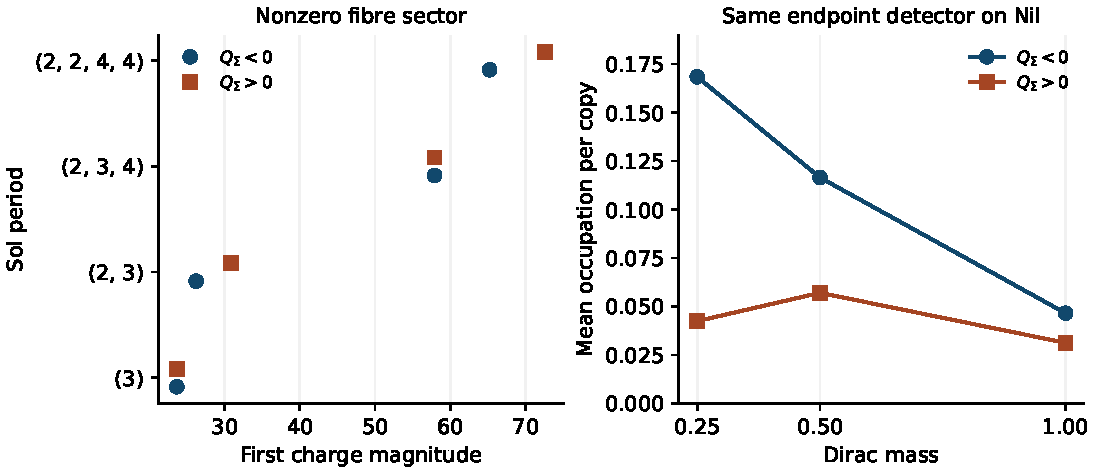
\includegraphics[width=\linewidth]{figures/readouts.pdf}
\caption{Two different comparisons. Left, the first nonzero-fibre charge magnitudes of four Sol lattices, plotted at the interval midpoints from Table~\ref{tab:sol}. Right, the particle-side mean for the same Nil shell and LC apparatus on each branch at three masses, \(h=0,\ |u|=3/8\). Lines join the calculated masses only.}
\label{fig:device}
\end{figure}

With \(m_D=0\), the massless paired two-band generator has charge dependence proportional to the identity within each Weyl block: after discarding its phase the Hamiltonian is \(\nu A\sigma_3+\sqrt{2\nu n}E\sigma_1\). A changing metric can still generate transitions, but their band probabilities are even under charge reversal. A sign-sensitive \emph{massive} finite-shell device and a massless even transition on the same space are compatible. The present calculation uses no infinite-mode Fock implementability assumption.

\section{Discussion}
A signed threshold can be read from a measured kernel when the allowed momentum sector, charge normalization, spin structure and metric are known. The theorem on Sol replaces the full first-gap equality problem by two integer minima for the reference metric and invariant spin lift. It does not reduce every higher signed gap to the two ground levels: period \((2,3)\) exhibits an excited-state competitor. The eta invariant is a global regularized quantity that can vanish even when these first levels split.

For a state observable one must also specify a mass, a preparation and a detector. The Nil apparatus compares two different propagators between the same projectors, so a difference is attributable to the charge within the prescribed model. A change of apparatus can change the ordering of occupations. For example at \(|u|=1/8,\ h=0,\ m_D=1\) the same lowest LC device gives approximately \(0.00823954\) and \(0.00824377\) in \(+u,-u\) order. The result supplies no universal choice of vacuum or probability law for the gravitational charge.

Several questions survive these examples. Beyond trace 60, is there a chiral cyclic monodromy with equal signed minima? For other Sol spin structures, a translated dual lattice can alter the arithmetic domain. On higher-genus Seifert bases, the missing input is the relevant twisted base Dirac spectrum. More generally a physical protocol would have to fix the charge magnitude or calibrate it independently of the sign. These questions concern different extensions of the stated sign tests.

\section*{Availability and acknowledgment}
The accompanying supplement contains the class register, certified intervals, spin-lift tables, finite-shell data, and stand-alone reproduction programs. English sources and a Japanese reading edition accompany this manuscript. OpenAI Codex assisted with manuscript preparation, translation and computational checks.
\appendix
\section{Connection and sign dictionary}\label{app:conv}
In an oriented orthonormal coframe the spatial part of the contortion \(K_{ij}=w\epsilon_{ijk}e^k\) gives \(T^i=K^i{}_j\wedge e^j=-2w\,e^{jk}\) cyclically. Thus the spatial pullback of \(e_a\wedge T^a\) is \(-6w\,e^{123}\). In the spin connection the ordered-pair sum of contortion terms gives \(-\tfrac14\sum_{ijk}w\epsilon_{ijk}c_kc_ic_j=3wI/2\) with our convention for connection indices. This calculation fixes the sign of the scalar shift before it is applied to any spectrum.

For clarity one can eliminate both isotropic torsion amplitudes before forming the spin operator. Write \(T^i=v e^{0i}+2j e^{jk}\) cyclically. Up to the common positive density and the factor \(1/\kappa^2\), the auxiliary part of the homogeneous Lagrangian is
\[
 3(-j^2+v^2+2hvj)-6\kappa^2\dot\theta j .
\]
The two stationary equations give \(v=-hj,\ j=-\kappa^2\dot\theta/(1+h^2)\) and \(w=-j\). The fixed-charge endpoint term follows by a Legendre transformation. On the minimal branch the tensor part vanishes by the invertible Cartan equation. The real Holst term mixes the vector and axial parts through a matrix with determinant proportional to \(1+h^2>0\); its trace piece drops out of the symmetrized Hermitian Dirac action, whose contortion anticommutator projects onto the completely antisymmetric component. The reduced kinetic density is \(3\kappa^2\dot\theta^2/d\). Its momentum on the slice is \(6\kappa^2\vol\dot\theta/d\), in agreement with \(-Q_\Sigma\).

For \(\vol=V_0W\), \(w=u/W,\ u=-Q_\Sigma/(6V_0)\), whereas the raw scalar velocity constant is \(\kappa^2 W\dot\theta=d u\). Ratios referred to \(+u\) in the transport data refer to \emph{negative} \(Q_\Sigma\). Sections on spherical geometry use the dimensionless operator \(qD=D_{\rm unit}-sX\) for charge sign \(s\) and \(X\ge0\). Reversing orientation and the associated spin lift exchanges the two signed spectra and reverses ordinary eta. The lens row in Appendix~\ref{app:spheres} and the cyclic coordinate convention in Appendix~\ref{app:energy} are related by this reversal for \(L(7,2)\).

\section{Arithmetic enumeration and certified Sol intervals}\label{app:enumerate}
\subsection{A bounded integer search with a proof of completeness}
The free product presentation \(PSL_2(\Z)=C_2*C_3\) identifies primitive hyperbolic conjugacy classes with primitive mixed positive \(L,R\) necklaces. In a cyclically reduced word the two choices of exponent of the order-three factor give the two letters. A trace-positive lift is unique. Every mixed word can start at an \(LR\) pair. Appending \(L\) or \(R\) to its positive matrix increases the trace by a positive off-diagonal entry. A search tree can consequently be cut as soon as its trace exceeds 60; taking one cyclic representative and removing proper powers yields the finite list without a word-length assumption. For \(B(b)=\left(\begin{smallmatrix}b&-1\\1&0\end{smallmatrix}\right)\) one has \(L^{-1}B(b)L=L^{b-2}R\), giving the advertised periods and an integral change of basis.

For each representative, put \(S=2br+(d_0-a)s\). Completing the square in \eqref{eq:F} gives \(4bF=S^2-\Delta s^2\). Multiplication by \(M^\mathsf T\) rescales \(S+\sqrt{\Delta}s\) by one of \(e^{\pm\ell}\). Each orbit has exactly one representative with
\[
 e^{-\ell}\le (S+\sqrt\Delta s)^2/(4b|F|)<e^\ell .
\]
The two coordinate unit vectors show that it suffices to search \(|F|\le m_0=\max(b,c)\). Bounding the sum and difference of the two embeddings within this fundamental domain gives
\[
 |S|\le2\sqrt{bm_0t},\qquad |s|\le2\sqrt{bm_0t/\Delta}.
\]
Enumerate the integer rectangle and retain \(S\equiv(d_0-a)s\bmod 2b\). Boundary inequalities use the sign of \(p+q\sqrt\Delta\), obtained by comparing integer squares when the terms have opposite signs. Vectors \(v,-v\) are different oriented orbits. This matters, for example, for the multiplicity four in Table~\ref{tab:sol}. A sample independent count occurs on the golden-ratio lattice: identifying the dual lattice with \(\Z[\varphi]\), \(\varphi=(1+\sqrt5)/2\), the monodromy multiplies by \(\varphi^2\). The Minkowski bound \(\sqrt5/2<2\) makes every ideal principal. The four unit cosets modulo \(\langle\varphi^2\rangle\) give four orbits per ideal of absolute norm \(n\); precisely two have each sign. The number of oriented orbits is \(4\sum_{d\mid n}\chi_5(d)\) for the real quadratic character \(\chi_5\).

For the golden-ratio lattice the first level can also be bracketed without a Hermite expansion. In the \(|F|=1\) sector oscillator comparison gives a squared ground lower bound \(35.6460\) and second-level lower bound \(47.5306\). A width-nine Gaussian with central potential in its lower spin eigendirection gives the squared ground upper bound \(37.8506\); all higher norms start above \(62.2175\). Multiplying the resulting absolute-level interval by \(4\ell\) gives \(22.9843<q_\pm<23.6845\) with two copies on each branch. The first row of Table~\ref{tab:sol} refines this independent bracket.

\subsection{Eta and the framing}
The Sol invariant frame is globally defined for our trivial deck spin character. The Levi--Civita spin connection contribution to the spin Dirac operator cancels in this frame. On even forms, write a section as \((f,*v)\). The signature operator formed using the flat framing connection acts in the corresponding quaternion frame by the same three coefficient derivatives and Clifford matrices, with complex volume element of the same sign. Complexifying the quaternionic module gives two equivalent two-dimensional spin representations. Their domains agree on the compact quotient because the frame and the deck character are trivial. Its eta is therefore \(2\eta_D\). The cusp signature-defect formula of Atiyah--Donnelly--Singer \cite{ads}, Atiyah's hyperbolic matrix invariant \cite{atiyah} and Hirzebruch's period formula \cite{hirz} identify this framed value with \(\sum_j(b_j-3)/3\), with the orientation calibrated by \(F=r^2-3s^2\) on the discriminant-12 lattice. The zero-fibre spectrum is paired. No termwise summation of individual orbit eta values at zero is involved. For example \((2,3)\) gives \(-1/6\); a mirror changes its sign.

\subsection{Full-line error and level isolation}
In a fixed rotated spin basis, for positive \(km\),
\[
 D_B=-i\sigma_2\partial_\xi+B\cosh\xi\,\sigma_3+B\sinh\xi\,\sigma_1,\qquad
 D_B^2=-\partial_\xi^2+B^2\cosh(2\xi)+B(-\cosh\xi\,\sigma_3+\sinh\xi\,\sigma_1).
\]
The pointwise norm of the last matrix divided by \(B\) is \(\sqrt{\cosh(2\xi)}\). For \(B>1/2\) the derivative of the squared form is bounded below by \(2B-1>0\). All ordered squared levels thus increase in the finite survey, where \(B\ge2\pi\sqrt{2/\sqrt{60^2-4}}>1/2\). This extra result controls possible competing excitations in the four examples. The unrestricted theorem needs only Lemma~\ref{lem:ground}.

Let \(\delta=7/50,\ \omega=B\sqrt{2(1-\delta)}\). The spin potential minus its value at zero has norm at most \(B\sqrt{\cosh(2\xi)-1}\). Using Young's inequality and \(\cosh(2\xi)\ge1+2\xi^2\) gives
\[
 D_B^2\ \ge\ -\partial_\xi^2+\omega^2\xi^2+B^2-\frac1{4\delta}-B\sigma_3 .
\]
The oscillator comparison gives lower bounds for the second and third eigenvalues, in increasing order adding \(+B+\omega,-B+3\omega\) to the scalar constant. For a normalized trial spinor \(v\), \(m=\langle D_B\rangle_v\), the spectral theorem puts an eigenvalue in \([m-r,m+r]\), \(r^2=\langle D_B^2\rangle_v-m^2\). We use 20 Hermite functions per spin, Gaussian width seven, and integer coefficient vectors selected numerically; only the integer vectors and full-line Gaussian moments enter the enclosure. The first interval lies below the second squared lower bound, and both disjoint intervals lie below the third squared lower bound. Min--max and simplicity then identify their index and sign. Multiplication by \(4\ell\) converts them to Table~\ref{tab:sol}. The residual uses the true square on the full line, including components outside the trial subspace.

\section{Round spin lifts and first-shell convention}\label{app:spheres}
Take \(S^3\) with the convention in which the constant invariant-frame doublet on a left quotient descends in the first positive shell. For a left action with lift character \(\chi\) on a finite subgroup \(G\), the invariant dimensions from Section~\ref{sec:catalog} specialize to
\[
 m_+(k)=(k+2)\dim(V_k\otimes\chi)^G,\qquad
 m_-(k)=(k+1)\dim(V_{k+1}\otimes\chi)^G .
\]
For a mixed cyclic action with two \(SU(2)\) weights \(a,b\) modulo \(p\), count the pairs \(u=-i,-i+2,\dots,i,\ v=-j,-j+2,\dots,j\) satisfying \(au+bv=0\bmod p\). Call this integer \(N(i,j)\); then \(m_+(k)=N(k,k+1)\), \(m_-(k)=N(k+1,k)\).

\begin{center}\small
\begin{tabular}{@{}llrrr@{}}\toprule
Quotient & Lift & \(m_+(0)\)& \(m_-(0)\)& \(\eta_0\)\\\midrule
\(S^3\) & unique &2&2&0\\
\(\mathbb{RP}^3\) & even / odd &2 / 0&0 / 2&\(1/4,\ -1/4\)\\
\(C_3\) quotient & left / right &2 / 0&0 / 2&\(4/9,\ -4/9\)\\
\(L(5,2)\) & \((a,b)=(2,1)\) &0&0&0\\
\(L(7,2)\), chosen orientation & \((3,2)\) &0&0&\(4/7\)\\
Binary tetrahedral \(2T\)&trivial&2&0&\(167/144\)\\
Binary octahedral \(2O\)&trivial / sign&2 / 0&0 / 0&\(383/288,\ -49/288\)\\
Binary icosahedral \(2I\)&trivial&2&0&\(1079/720\)\\
Quaternion \(Q_8\)&trivial&2&0&\(13/16\)\\
Quaternion \(Q_8\)&three nontrivial&0&0&\(-3/16\) each\\\bottomrule
\end{tabular}
\end{center}
These 15 entries refer to three-dimensional ordinary eta. For the binary groups the character average uses \(\sin((k+1)\theta)/\sin\theta\) away from the two central elements and the limiting signed dimension at those elements. Each residue of \(p_k=m_+(k)-m_-(k)\) modulo a group period \(P\) is a polynomial of degree at most two in \(k\). Thus \(\sum p_k z^k=N(z)/(1-z^P)^3\); the first \(3P\) differences determine \(N\). The unpaired identity contribution vanishes, and free action makes the nonidentity generating functions regular at \(z=1\). In particular \(N(1)=N'(1)=N''(1)=0\), and the finite Abel value \(-N'''(1)/(6P^3)\) gives the ordinary eta at zero by Mellin continuation. The stored coefficients allow all shell differences to be reconstructed; the script evaluates the integer dimensions before regularization. Four-dimensional boundary domains and determinant powers require separate data.

\section{Nil spectra and the eta correction}\label{app:nil}
Use horizontal lattice period \(P=2\pi\), central period \(P^2/r\) and volume \(V_0W=P^4a^2c/r\). For a general physical scalar shift \(\mu\) the spectral centre is \(b_0=\mu-t/4,\ t=c/a^2\). On the center-zero sector (present only if \(\delta_3=0\)) the levels about \(b_0\) are \(\pm|\boldsymbol l|/a,\ \boldsymbol l\in\Z^2+(\delta_1,\delta_2)\), retaining both dimensions when \(\boldsymbol l=0\). On a nonzero central frequency \(k=r|j+\delta_3|\), \(\nu=k/(2\pi)\), the remaining levels about \(b_0\) are
\[
 f=-\nu/c,\qquad f_n^\pm=\pm\sqrt{(\nu/c)^2+2\nu n/a^2},\quad n\ge1.
\]
Each occurs with multiplicity \(2k\) including both centre signs. Indeed Fourier expansion in the centre turns horizontal Clifford differentiation into an oscillator raising/lowering pair. The adjacent Hermite degrees span a two-dimensional block with diagonal \(\pm\nu/c\) and off-diagonal \(\sqrt{2\nu n}/a\). The remaining unpaired vector has eigenvalue \(-\nu/c\). Translation by one horizontal period shifts the second Fourier label by \(k\) and leaves \(k\) independent residue classes for each centre sign. Minimizing the paired positive and unpaired negative towers proves \eqref{eq:nilmin} where its gap assumptions hold. The equality point follows by squaring \(R_*=\nu_*/t+t/2\).

The nonzero-centre spin area term \(-t/4\) follows from the Koszul connection. To compare eta with \cite[Thm.~12]{gornet}, set the geometric parameters there to \(A_{\rm GR}=1/t,\ r_{\rm GR}=P^2c/r,\ m_v=r\). At the centred shift \(\mu=t/4\) the paired towers cancel. The unpaired value \(-2r\zeta(-1,\alpha)\) equals \(C_r=r/6\) for \(\alpha=1\) (periodic), \(-r/12\) for \(\alpha=1/2\). The local heat coefficient gives the smooth derivative \(\partial_\mu\eta_{\rm sm}=\vol(R_3/24-\mu^2)/\pi^2,\ R_3=-t^2/2\). Adding the signed crossings yields
\begin{align*}
 \eta(\mu)&=C_r+\frac{\vol}{\pi^2}\left(\frac{(t/4)^3-\mu^3}{3}
                     +\frac{(\mu-t/4)R_3}{24}\right)+J,\\
 J&=\sum_f d_f\{\sgn(f+\mu-t/4)-\sgn f\},\qquad \sgn(0)=0 .
\end{align*}
The finite sum contains only \(|f|\le|\mu-t/4|\). At \(\mu=0\) the smooth term equals \(\vol t^3/(96\pi^2)\). The horizontal contribution to \(J\) exists only for a central-periodic spin. At \(a=c=1,r=2,(\delta_1,\delta_2)=(0,1/2)\), the ordinary eta values are about \(1.15580037\) and \(0.65580037\) for the two central spins, both positive despite the sign change of \(C_r\).

\section{Flat lifts and critical lengths}\label{app:flat}
Take square horizontal lattices for \(m=2,4\) and unit-edge hexagonal ones for \(m=3,6\). Let periodicity of a spinor under the three translations be \((-1)^i,(-1)^j,(-1)^k\). A right screw of angle \(2\pi/m\) and axial displacement \(L/m\) lifts as \(s\exp(-i\pi\sigma_3/m)\), \(s=\pm1\); thus \((-1)^k=-s^m\). The horizontal character must be rotation-invariant. There are four options for order two, two for order four, and one each for orders three and six. On the order-four manifold the two nonperiodic-horizontal lifts have paired spectra; on the Hantzsche--Wendt manifold all four spins have half-integral momenta in each direction and every orbit is paired. Only the fully periodic three-torus has a two-dimensional unshifted kernel.

For horizontal-periodic spin solve \(e^{2\pi iz/m}=s e^{\mp i\pi/m}\) along each axial eigenspinor. Both lines give the same axial tower with
\(c_*=(-\tfrac12+\tfrac m2\,\mathbf1_{s=-1})\bmod m\). The two Hurwitz zeta values at zero give the eta formula in Section~\ref{sec:catalog}. The pairs in \(s=+,-\) order are \((-1,1)\), \((-4/3,2/3)\), \((-3/2,1/2)\), \((-5/3,1/3)\) for \(m=2,3,4,6\). Pf\"affle's axial tower uses the opposite operator sign \cite[Thms.~5.4, 5.6]{pfaffle}; changing it once matches all eight nonzero values. The 20 remaining lifts have zero eta.

For a nonaxial mode the screw rotates the horizontal covector through its full orbit and leaves each sign once per orbit. Let \(z_0=k/2\) with translation bit \(k=0,1\). Comparing its minimum against the two axial levels gives splitting precisely when
\[
 L^2>(\min(c_*,m-c_*)^2-z_0^2)/\rho^2
\]
for the asymmetric lifts. At equality one should add multiplicities of any tied shells on each side. For \(m=6,s=-1\), \(\rho=2/\sqrt3,\ z_0=1/2,\ c_*=5/2\); the critical \(L^2\) is \(9/2\). Translation and screw lifts thus supply both the first-gap equality and its breakdown in a single metric family. Numerical charge units use \(q_\pm=4\vol|\lambda_\pm|\), including the holonomy quotient in the volume.

\section{Product projections and a Seifert control}\label{app:product}
On the product with sphere radius \(a\) and longitudinal scale \(b\), use
\(D=D_2/a+\Gamma(-i\partial_\chi)/b\),
\(D_2=\sigma\cdot{\bf L}+1,\ \Gamma=\sigma\cdot x,\ \{\Gamma,D_2\}=0\).
For integer \(m\ge1\) the spherical levels \(\pm m\) have multiplicity \(2m\) and orbital angular momenta \(m-1,m\), respectively. At circle momentum \(p=2\pi(n+\delta)/L\) the two signs have modulus \(\sqrt{m^2/a^2+p^2/b^2}\). On the product both circle spins therefore give zero eta. On the connected-sum quotient, the two involutions combine the antipodal pullback with reflections \(\chi\mapsto-\chi,L-\chi\) and spin signs \(e_\alpha,e_\beta\). Their product gives circle parity \(e_\alpha e_\beta\). Each paired \(p,-p\) sector with \(p>0\) contributes equally to the two signs. The \(p=0\) sector exists only for \(e_\alpha=e_\beta\), and keeps orbital angular momentum \(l\) with \(e_\alpha(-1)^l=1\). Its levels are \(e_\alpha(-1)^{m-1}m/a\) with multiplicity \(2m\). Thus
\[
 \eta_D(z)=2e_\alpha a^z(1-2^{2-z})\zeta(z-1),\qquad \eta_D(0)=e_\alpha/2.
\]
The other two lifts have zero eta.

For the Seifert comparison the reference link orientation agrees with the positive invariant doublet of the left \(2I\) quotient. The spherical cover has radius two; the \(M(2,3,6)\) circle has length \(2\pi\) over a hexagonal torus of area \(2\pi\); on \(M(2,3,7)\) the circle length is \(2\pi\) over the curvature-minus-one \((2,3,7)\) orbifold. These are the unit-aspect choices for the values quoted in Section~\ref{sec:catalog}. The associated framed Pontryagin Chern--Simons integrals are \(1/60,1/2,5/84\), respectively. When no crossing occurs the ordinary Dirac eta change is minus one twelfth of the change in this integral. The integer reference part depends on the spin lift and the vertical tower; general adiabatic Seifert techniques appear in \cite{nicolaescu}. For \(M(2,3,7)\) the reference limit is \(-925/504\); subtracting \( (5/84)/12\) gives \(-1853/1008\). These benchmarks are used solely for comparison. They do not determine the least base-dependent Dirac level of a general Seifert quotient.

\section{An all-order criterion for the first lens-shell interval}\label{app:energy}
Let the action on the two complex coordinates have rotation weights \((1,r)\) modulo \(p\), \(\gcd(r,p)=1\). For each \(t=0,1\) obeying \(1+r+tp=0\bmod2\), put \(a=(1+r+tp)/2,\ b=(1-r+tp)/2\). Then \(m_+(0)=2\mathbf1_{b=0\bmod p}\) and \(m_-(0)=2\mathbf1_{a=0\bmod p}\). For \(p\ge2\) at most one side has a first-shell doublet. Changing \(r\) to \(-r\) exchanges \(a,b\) and reverses the eta sign. In this generator convention \(L(7,2)\) has \((a,b)=(5,3)\), \(\eta_0=-4/7\), the mirror of the row with \(+4/7\) in Appendix~\ref{app:spheres}.

When \(\delta_0\ne0\), the finite group acts in one \(SU(2)\) factor only. The character formula reduces to an elementary sum whose sign is that of \(\delta_0\):
\[
 \frac{\eta_0}{\delta_0}=\frac1p\sum_{j=1}^{p-1}
                 \frac1{2-2\cos(2\pi j/p)}=\frac{p^2-1}{12p}.
\]
The last identity follows from logarithmic derivatives of \((z^p-1)/(z-1)\) at \(z=1\). Setting \eqref{eq:energy} to zero gives \(X_*=3/[2(1-\eta_0/\delta_0)]\); an interior zero requires \(0<\eta_0/\delta_0<2/5\). Exactly \(p=2,3,4\) satisfy it. When \(\delta_0=0\), \(D=2X\eta_0\) is identically zero in this interval or has no zero there. For \(L(7,2)\) the next-shell imbalance gives the first positive zero at \(7/2\); both mirror conventions have that position. The finite register contains six lifts with isolated first-interval zeros, ten identically zero there and 418 without an interior zero.

\section{Validated finite-shell propagation}\label{app:device}
The lowest unpaired Nil tower shifts by \(-\nu/c\) from the spectral centre. Multiplication by \(W\) converts this term to \(-\nu a^2\), the scalar part to \(3u/2-c^2/4\), and the physical mass to \(m_DW\). This derives \eqref{eq:device}, including the axial charge sign, directly from the adjacent-mode reduction. In a fixed two-component basis define \(z_0=-c^2/4-\nu a^2\) and \(x=m_D W>0\). Each LC projector is \(\tfrac12[I\pm(x\sigma_1+z_0\sigma_3)/\sqrt{x^2+z_0^2}]\) evaluated at its endpoint. The \(k=1\) shell has two central copies but equation~\eqref{eq:occup} acts on a single copy.

For a smooth Hermitian \(H\) on a step of width \(\delta\) compare the true propagator with \(\exp[-i\delta H(s_{\rm mid})]\). In the Duhamel formula subtract the term linear in \(s-s_{\rm mid}\) with endpoint factors frozen, whose midpoint integral vanishes. The second Taylor remainder integrates to \(\delta^3\sup\|H''\|/24\); bounding the variation of the unitary factors multiplying the first derivative gives \(\delta^3\sup\|H\|\sup\|H'\|/6\). Since each factor is unitary, local norm errors add directly across the 4096 equal steps. An accumulated propagator error \(\epsilon\) changes the squared rank-one amplitude by at most \(2\epsilon+\epsilon^2\). Derivatives of \eqref{eq:nilhistory} and Pauli exponentials are enclosed with 90-bit Arb arithmetic. For the chosen \(h=0\) device the resulting rounded boxes are
\[
 \begin{array}{ll}
 n_{u>0}=0.16845\ \pm2.83\times10^{-6},&n_{u<0}=0.04248\ \pm6.89\times10^{-6},\\
 n_{u>0}-n_{u<0}=0.12598\ \pm8.18\times10^{-6},&
 n_{u>0}/n_{u<0}=3.966\ \pm3.85\times10^{-4}.
 \end{array}
\]
The separately integrated high-accuracy ODE values quoted in the text fall inside these enclosures. For \(h=1\), fixed \(u\) and the same two LC endpoint definitions, the ratio is \(3.14\pm0.00235\). The closed formula for the metric changes with \(h\). A detector built from fixed left/right component projectors also defines a consistent measurement but gives different values. There is no sum over all ultraviolet modes in these error estimates.

\section{Reproducing the numbers and their scope}
From the root of the supplement install the packages in \texttt{script/requirements.txt}. Run \texttt{python -B script/paper08.py verify} to check the published data and \texttt{python -B script/paper08.py recompute --output results} to repeat the calculations into a new directory. The public computation enumerates Sol necklaces and signed minima, reconstructs whole-line test-vector certificates, obtains all fifteen spherical lift character series and the 434 lens entries, generates the 28 flat spectra and 72 Nil reference leaves, and propagates and bounds the representative finite-shell occupations. Rendering reads these outputs directly. The integer arithmetic and error enclosures have different roles: rounded eigenvectors suggest trials; their integerized coefficients enter rigorous integrals. An ODE estimate of a probability and an interval bound on the same probability are retained separately.

Numerical agreement is evidence for the stated formulas on their sampled domains. The split criterion outside trace 60 is an operator theorem; the numerical census of topological chirality covers only the stated traces. For the spin Dirac spectrum on the centred Nil slice, reversing the central spin changes the sign of the constant \(C_r\); the actual eta also includes metric and crossing terms. On Sol a negative-norm unit suffices for one reversal type; another reversal can exist without such a unit. On the connected sum of projective spaces there are two nonzero ordinary eta values of opposite signs even though the manifold admits orientation reversal. These distinctions are needed to reproduce the interpretations as well as the numerical tables.

\begin{thebibliography}{99}
\bibitem{p04} Muacca, \emph{Kaluza--Klein Quadratic Forms and Torsion Boundary Data on Four Compact Geometries}, DPPU Paper 04, v2 (2026). \href{https://doi.org/10.5281/zenodo.19775695}{Source}.
\bibitem{p07} Muacca, \emph{Lorentzian Einstein--Cartan Reduction on Compact Homogeneous Geometries: Constraints and Inhomogeneous Perturbations}, DPPU Paper 07, v2 (2026). \href{https://doi.org/10.5281/zenodo.20678646}{Source}.
\bibitem{calcagni} G. Calcagni and S. Mercuri, \emph{Barbero--Immirzi field in canonical formalism of pure gravity}, Phys. Rev. D 79, 084004 (2009). \href{https://arxiv.org/abs/0902.0957}{Source}.
\bibitem{ammann} B. Ammann and C. B\"ar, \emph{The Dirac operator on nilmanifolds and collapsing circle bundles}, arXiv:math/9801091. \href{https://arxiv.org/abs/math/9801091}{Source}.
\bibitem{gornet} R. Gornet and K. Richardson, \emph{The eta invariant on two-step nilmanifolds}, arXiv:1210.8070v5 (2024). \href{https://arxiv.org/abs/1210.8070v5}{Source}.
\bibitem{pfaffle} F. Pf\"affle, \emph{The Dirac spectrum of Bieberbach manifolds}, J. Geom. Phys. 35 (2000), 367--385. \href{https://www.sciencedirect.com/science/article/pii/S039304400000005X}{Source}.
\bibitem{baer} C. B\"ar, \emph{The Dirac operator on space forms of positive curvature}, J. Math. Soc. Japan 48 (1996), 69--83. \href{https://www.jstage.jst.go.jp/article/jmath1948/48/1/48_1_69/_article/-char/en}{Source}.
\bibitem{boldt} S. Boldt and E. A. Lauret, \emph{An explicit formula for the Dirac multiplicities on lens spaces}, J. Geom. Anal. 27 (2017), 689--725. \href{https://arxiv.org/abs/1412.2599}{Source}.
\bibitem{lin} F. Lin, \emph{Monopole Floer homology and SOLV geometry}, Ann. Henri Lebesgue 3 (2020), 1117--1131. \href{https://doi.org/10.5802/ahl.56}{Source}.
\bibitem{marcolli} M. Marcolli, \emph{Solvmanifolds and noncommutative tori with real multiplication}, arXiv:0711.2036. \href{https://arxiv.org/abs/0711.2036}{Source}.
\bibitem{bolsinov} A. V. Bolsinov, H. R. Dullin and A. P. Veselov, \emph{Spectra of Sol-manifolds: arithmetic and quantum monodromy}, arXiv:math-ph/0503046. \href{https://arxiv.org/abs/math-ph/0503046}{Source}.
\bibitem{ads} M. F. Atiyah, H. Donnelly and I. M. Singer, \emph{Eta invariants, signature defects of cusps, and values of \(L\)-functions}, Ann. of Math. 118 (1983), 131--177. \href{https://annals.math.princeton.edu/1983/118-1/p08}{Source}.
\bibitem{atiyah} M. F. Atiyah, \emph{The logarithm of the Dedekind \(\eta\)-function}, Math. Ann. 278 (1987), 335--380. \href{https://webhomes.maths.ed.ac.uk/~v1ranick/papers/atiyahlg.pdf}{Source}.
\bibitem{hirz} F. Hirzebruch, \emph{Hilbert modular surfaces}, L'Enseignement Math\'ematique 19 (1973), 183--281. \href{https://webhomes.maths.ed.ac.uk/~v1ranick/papers/hirzhilb.pdf}{Source}.
\bibitem{nicolaescu} L. I. Nicolaescu, \emph{Finite energy Seiberg--Witten moduli spaces on 4-manifolds bounding Seifert fibrations}, arXiv:dg-ga/9711006. \href{https://arxiv.org/abs/dg-ga/9711006}{Source}.
\end{thebibliography}

\end{document}
